% !TEX program = xelatex

\documentclass{resume}
\usepackage{graphicx}
\usepackage{tabu}
\usepackage{multirow}
%\usepackage{zh_CN-Adobefonts_external} % Simplified Chinese Support using external fonts (./fonts/zh_CN-Adobe/)
%\usepackage{zh_CN-Adobefonts_internal} % Simplified Chinese Support using system fonts

\begin{document}
\pagenumbering{gobble} % suppress displaying page number

\Large{
  \begin{tabu}{ c l r }
   \multirow{5}{1in}{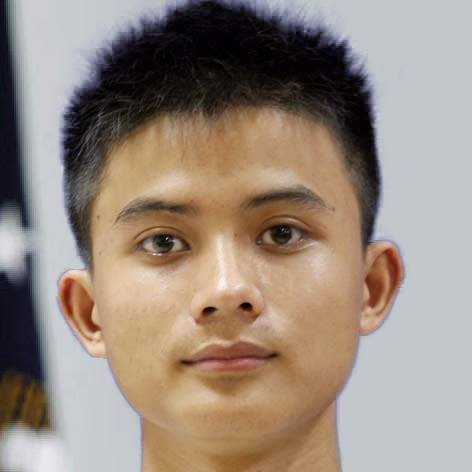
\includegraphics[width=0.88in]{avatar}} & \scshape{Toan Dao Minh}  \\
    & \email{toandaominh1997@gmail.com}  \\
    & \phone{(+84) 345-153-946}  \\
    & \linkedin[toaddaominh1997]{https://www.linkedin.com/in/toandaominh1997}  \\
    & \github[github.com/toandaominh1997]{https://github.com/toandaominh1997} 
  \end{tabu}
}

\section{\faHeartO Summary}
Machine Learning, Deep Learning, Computer Vision, Algorithms, Data structures, Competitive Programming
Data Mining, Software Engineering, Game Developper.


\section{\faGraduationCap\ Education}
\datedsubsection{\textbf{Ho Chi Minh City University of Science(HCMUS)},Vietnam National University}{2015 -- Present}
\textit{Currenttly pursuing B.S.E} in Computer Science, expected March 2019\\
\textbf{Course taken: }Functional Programming (Advanced), Algorithm Design and Data Structure (Advanced)
Calculus, Linear Algebra, Applied Statistic, Machine Learning, Digital Image Processing,
Data Mining, Infomation Retrieval, Object-oriented Programming, Programing Language
Operating System, Software Engineering
\section{\faUsers\ Experience}

\datedsubsection{\textbf{Gameloft} Ho chi minh city, Vietnam}{June. 2018 -- Dec. 2018}
\role{Game Developer}{Dungeon Hunter Champions}
Brief introduction: Dungeon Hunter Champions
\begin{itemize}
  \item Position: C++ Programmer
  \item Project Description: Game optimization/performance, 3D programming OPENGL, build the
Dungeon Hunter Champions game on Android using
bankend C++ via JNI on Java.

\end{itemize}

\datedsubsection{\textbf{FPT Software} Ho chi minh city, Vietnam}{Jan. 2018 -- June. 2018}
\role{Developer IOT}{Propose and development IoV system (Internet of vehicle)}
Brief introduction: Internet of vehicle
\begin{itemize}
  \item Client: Confidential
  \item Project size: 80 man-months
  \item Position: Software Engineering
  \item Responsibilities: Design system, find solution, and Coding module in automotive vehicles
  \item Project Description: Investigate and build IoV solution. Design and develop full system for customer.
\end{itemize}

\datedsubsection{\textbf{Kaggle Competitives Project}}{Sep. 2017 -- Present}
\role{Maintainer}{Individual Projects}
Brief introduction: Kaggle
\begin{itemize}
  \item Project Description: Build multiple models in Kaggle Challenge. By using multiple models: Supervised Learning, UnSupervised Learning, Deep Learning on scikit-learn, tensorflow, keras to solve challenge.
  \item Got into https://github.com/toandaominh1997/Kaggle.
\end{itemize}

\datedsubsection{\textbf{Surface Reconstruction 3D from 2D images Projects}}{Dec. 2017 -- Jan. 2018}
\role{Maintainer}{Individual Projects}
Brief introduction: Surface Reconstruction 3D from 2D images
\begin{itemize}
  \item Project Description: By using Poison Algorithms to 3D shaped reconstruction from a sequence of 2D images in Point Cloud Library.
\end{itemize}

\datedsubsection{\textbf{ Research and Install NXT Segway with Ride Projects}}{Oct. 2017 -- Jan. 2017}
\role{Maintainer}{Individual Projects}
Brief introduction: NXT Segway with Ride
\begin{itemize}
  \item Project Description: By using the NXT Color Sensor as a simple proximity sensor to the
ground to detect the approximate tilt angle of the robot, the robot can actually balance
itself!
\end{itemize}

% Reference Test
%\datedsubsection{\textbf{Paper Title\cite{zaharia2012resilient}}}{May. 2015}
%An xxx optimized for xxx\cite{verma2015large}
%\begin{itemize}
%  \item main contribution
%\end{itemize}

\section{\faCogs\ Skills}
\begin{itemize}[parsep=0.5ex]
  \item Algorithms: Especially good at mathematics, graph theories, data structures, and dynamic programming.
  \item Languages: C/C++, Java, Python. Familiar with Pascal, C#, Latex, HTML, CSS, Javascript.
  \item Technologies: Scikit-learn, Tensorflow, Keras, OpenCV, OpenGL, PCL(Point Cloud Library)
  \item Platforms: Windows, Linux, MacOS
  \item Software: Ms SQL Server, Android Studio, Git, Eclipse, Visual Studio, Vim, Emacs, NetBeans, Sublime Text


\end{itemize}

\section{\faHeartO\ Honors and Awards}
\datedline{\textit{Semi-finals}, SnackDown 2017 competition hosted by Codechef.com}{Mar. 2017}
\datedline{\textit{Rank 14/98 team}, ACM ICPC online of Postsand Telecommunications Institute of Technology}{Summer. 2017}
\datedline{\textit{27/132}, Thach Thuc 2018 host at HCMUS}{Mar. 2018}
\datedline{\textit{Round 2}, ACM ICPC 2017 VietNam Northern Provincial Contest}{Oct. 2017}
\datedline{\textit{Round 2},ACM ICPC 2017 VietNam Southern Provincial Contest.}{Oct. 2017}
\datedline{\textit{ Consolation Prize Student},Olympiad in Informatics of Ho Chi Minh City University of Science.}{Oct. 2017}
\datedline{\textit{Round 2},ACM ICPC 2018 VietNam Southern Provincial Contest.}{Oct. 2018}
\datedline{\textit{Round 3},ACM ICPC Vietnam National Round 2018 Online}{Nov. 2018}


\section{\faInfo\ Miscellaneous}
\begin{itemize}[parsep=0.5ex]
  \item GitHub: https://github.com/toandaominh1997
  \item Languages: English -Conversational, Vietnamese - Native speaker
\end{itemize}

%% Reference
%\newpage
%\bibliographystyle{IEEETran}
%\bibliography{mycite}
\end{document}
